\mode<article>
{
\usepackage{fullpage}
}

\mode<presentation>
{
  \usetheme{Boadilla}
  \usecolortheme{whale}
  \usecolortheme{lily}

  \setbeamercovered{transparent}
  \usefonttheme[onlymath]{serif}
}

\usepackage{calendar}
\usepackage{datenumber}



\title[Syllabus] % (optional, use only with long paper titles)
{\course~\coursename: Syllabus}

\author[\instructorshort]% (optional, use only with lots of authors)
{\instructorlong}

\institute[\instituteshort] % (optional, but mostly needed)
{\institutelong}
% - Use the \inst command only if there are several affiliations.
% - Keep it simple, no one is interested in your street address.

\date % (optional)
{Semester/Year: \semesteryear}


% If you have a file called "university-logo-filename.xxx", where xxx
% is a graphic format that can be processed by latex or pdflatex,
% resp., then you can add a logo as follows:

%\pgfdeclareimage[height=1.1cm]{university-logo}{UniversityLogo}
%\logo{\pgfuseimage{university-logo}}



% Delete this, if you do not want the table of contents to pop up at
% the beginning of each subsection:
%\AtBeginSection[]
%{
%  \begin{frame}<beamer>{Outline}
%    \tableofcontents[currentsection,currentsubsection]
%  \end{frame}
%}


% If you wish to uncover everything in a step-wise fashion, uncomment
% the following command:

%\beamerdefaultoverlayspecification{<+->}


\begin{document}

\begin{frame}
  \titlepage
\end{frame}

%\mode<presentation>{
%\begin{frame}{Outline}
%  \tableofcontents
%  % You might wish to add the option [pausesections]
%\end{frame}}

\mode<article>{
\maketitle
%\tableofcontents
}


\section{Syllabus}

\begin{frame}{Course Info}
\begin{itemize}
\item Class meeting schedule: 12:00AM - 1:15PM, Monday and Wednesday. 
\item Class location: Brown Building 304 and 305. 
\item Course Webpages:
\begin{itemize}
\item Blackboard (\url{http://blackboard.mines.edu/}). All current CSM students should have a blackboard account, and students registered for this course will be automatically enrolled. Check with CCIT if you do not have a blackboard account.
%\item {Piazza (\url{http://piazza.com/mines/spring2015/eeng307/home}). Piazza will be used as a QA forum for content and general questions.  (Preferred to email)}
\end{itemize}
\end{itemize}
\end{frame}

\begin{frame}{Instructors}
  \begin{itemize}
  \item Vibhuti Dave
  \begin{itemize}
  \item Office: BB314C
%  \item Office hours: MW 4:00-5:00pm
  \item Email: vdave@mines.edu
  \end{itemize}
  \item Tyrone Vincent
    \begin{itemize}
  \item Office: BB327D
%  \item Office hours: M 1:00-2:30pm, W 2:30-4:00pm
  \item Email: tvincent@mines.edu
  \end{itemize}
  \end{itemize}
\end{frame}

\begin{frame}{Course Assistants}
\begin{itemize}
\item Henry Dau
\begin{itemize}
\item Email: hdau@mymail.mines.edu
\end{itemize}
\item Jonathan Hong
\begin{itemize}
\item Email: jhong@mymail.mines.edu
\end{itemize}
\item Joel Kuenning
\begin{itemize}
\item Email: jkuennin@mymail.mines.edu
\end{itemize}
\item Joshua Nelson
\begin{itemize}
\item Email: josnelso@mymail.mines.edu
\end{itemize}
\end{itemize}
\end{frame}

\noindent\textbf{Instructional Activity:} 3 hours lab, 1 semester hours.\\

\noindent\textbf{Course designation:} Elective/Major Requirement (EE)\\

\noindent\textbf{Course description:}
\begin{quote}
This laboratory is a semester-long design and build activity centered around a challenge problem that varies from year to year. Solving this problem requires the design and prototyping of a complex system and utilizes concepts from multiple electrical engineering courses. Students work in intra-disciplinary teams, with students focusing on either embedded systems or  control systems.
\end{quote}


\begin{frame}{Objectives}
\begin{block}{Students will be able to:}
\begin{itemize}
\item Design and debug integrated systems as an intra-disciplinary team.
\item Design experiments and gather data to solve engineering problems and/or demonstrate performance of sub-systems or systems.
\item Predict the performance of a designed system and verify their predictions experimentally.
\item Work effectively in intra-disciplinary teams to solve engineering problems.
\item Engage in reflective learning and demonstrate an ability to engage in life-long learning.
\end{itemize}
\end{block}
\end{frame}

\begin{frame}{Section Specific Objectives:}{Embedded Systems}
\begin{block}{Students will be able to:}
\begin{itemize}
\item  Interface various kinds of sensors to a microcontroller.
\item  Use a microcontroller to drive and control  motors. 
\item  Implement communication between processors using wired and wireless protocols.
\item  Design a user interface to enable a human being to interact with their integrated system.
\item  Exploit built-in features within a microcontroller such as ADCs, DACs, and timers to design an efficient system.
\end{itemize}
\end{block}
\end{frame}


\begin{frame}{Section Specific Objectives:}{Control Systems}
\begin{block}{Students will be able to:}
\begin{itemize}
\item Use Simulink to model a dynamic system.
\item Design and execute experiments to find unknown parameters describing a dynamic system.
\item Design and implement a PI controller to regulate the speed of a motor.
\item Design and implement a controller to stabilize an inverted pendulum.
\item Design and implement a controller to regulate the horizontal position of a balancing robot.
\end{itemize}
\end{block}
\end{frame}

\begin{frame}{Project Description}
Your employer has determined that a highly maneuverable robot with small footprint that can carry items from one location to another has a viable market for sale to hospitals and in other institutional settings. Your team is assigned to design and build a prototype device, which is a two-wheeled balancing robot that can cary cargo to a desired destination. This prototype should be self balancing, and able to move in a straight line. While many balancing robots use a complete inertial measurement unit (IMU) that incorporates a gyrometer, accelerometer, and compass, these sensors are quite expensive. Your boss has asked you to balance using the robot using {\em only} a gyrometer, which measures angular velocity. Other available sensors are wheel encoders, line sensors, and ultrasonic sensors. It should be able to receive commands wirelessly, which include: stop and hold position, move forward, and move to target. The robot should also be able to detect obstacles and stop if detected.  For the demonstrations, the cargo will be a 0.5 liter or 1 liter water bottle filled with water. 
\end{frame}

\mode<article>{For convenience, some aspects of the design have been fixed: the motors, wheels, battery size, available sensors, and available embedded processors. However, you are free to choose all other elements of the design, including the construction of the robot frame (within the available Actobotics elements) placement of elements on the frame, and of course, all control systems, signal processing, and embedded system implementation.  
}

\mode<beamer>{\begin{frame}{Project Description}
For convenience, some aspects of the design have been fixed: the motors, wheels, battery size, available sensors, and available embedded processors. However, you are free to choose all other elements of the design, including the construction of the robot frame (within the available Actobotics elements) placement of elements on the frame, and of course, all control systems, signal processing, and embedded system implementation.  
\end{frame}}

\begin{frame}{Group Work}
You will be working in groups to complete the activities in this lab. This is done for several reasons. Researchers have shown that students that students working in small groups tend to learn more of what is taught and retain it longer than when the same content is presented in other instructional formats. In addition, the ability to work in a diverse group is an educational objective in itself, and one of the student outcomes that we are required to measure for accreditation of the electrical engineering degree is the ability to function on multidisciplinary teams. 

We will model a multidisciplinary team by having some members concentrate on embedded systems, and some members concentrate on control systems. Even though you are all electrical engineers, you will need to learn how to cooperate and communicate with team members whose expertise is different from yours. 
\end{frame}

\mode<article>{In order to assist in the formation and monitoring of the teams, we will use the CATME website. You will also be using CATME when you are in senior design. You will first fill out a team maker questionnaire with information about your background and skills.  We will then use CATME to form balanced teams. Before each demonstration, you will use CATME to fill out an evaluation of your team members. This will allow us to give feedback to you as to how you are working within the group. }


\mode<beamer>{\begin{frame}{Group Work}
In order to assist in the formation and monitoring of the teams, we will use the CATME website. You will also be using CATME when you are in senior design. You will first fill out a team maker questionnaire with information about your background and skills.  We will then use CATME to form balanced teams. Before each demonstration, you will use CATME to fill out an evaluation of your team members. This will allow us to give feedback to you as to how you are working within the group. 
\end{frame}}


\begin{frame}{Work Process}
Although we will be meeting in lab for 3 hours a week, it is expected that you will be working outside of lab as well to complete this course. You should plan on at least 1 hour of work outside of lab for every 1 hour in lab, plus additional time for meetings and communicating with your group members.

On blackboard, you will find a short document from the Derek Bok Center for Teaching and Learning, Harvard University, on best practices for working in groups. All students are expected to have read this document and are ready to participate in their groups once they are assigned. 
\end{frame}

\begin{frame}{Lab Availability/Office Hours}

%----------------------------------------------------------------------------------------

\begin{calendar}{\hsize}


%----------------------------------------------------------------------------------------
%	Monday
%----------------------------------------------------------------------------------------

\day{}{
\textbf{11:30am-12:00pm} \daysep Joel Kuenning Office Hours \\
\textbf{12:00pm-1:30pm} \daysep SEED Lab \hspace{.5in} \\
\textbf{1:30pm-3:00pm} \daysep Joel Kuenning Office Hours \\
\textbf{3:00pm-5:00pm} \daysep Joshua Nelson Office Hours \\
} 

%----------------------------------------------------------------------------------------
%	Tuesday
%----------------------------------------------------------------------------------------

\day{}{ Lab Not Available} 

%----------------------------------------------------------------------------------------
%	Wednesday
%----------------------------------------------------------------------------------------

\day{}{ % Wednesday
\textbf{11:00am-12:00pm} \daysep Jonathan Hong Office Hours\\
\textbf{12:00pm-1:30pm} \daysep SEED Lab \hspace{.5in} \\
\textbf{1:30pm-2:00pm} \daysep Jonathan Hong Office Hours \\
\textbf{3:00pm-5:00pm} \daysep Henry Dau Office Hours \\
\textbf{4:00pm-5:00pm} \daysep SEED Lab Debrief
} 

%----------------------------------------------------------------------------------------
%	Thursday
%----------------------------------------------------------------------------------------

\day{}{ Lab Not Available} 

%----------------------------------------------------------------------------------------
%	Friday
%----------------------------------------------------------------------------------------

\day{}{ % Friday
%\\
} 


%----------------------------------------------------------------------------------------
 
\finishCalendar
\end{calendar}
\end{frame}

\begin{frame}{Grading Scale}
Teams earn points up to the total listed in the grading scale below.
\begin{center}
\begin{block}{Available Points}
\begin{tabular}[t]{ccc}
Stage & Assignment & Points \\\hline
Aruino Intro & Documentation & 50 points \\\hline
Preliminaries & Documentation & 150 points \\\hline
\multirow{2}{*}{Demo 1}  & Documentation &200 points \\
& Performance & 100 points \\\hline
\multirow{2}{*}{Demo 2} & Documentation & 100 points \\
& Performance  & 150 points \\\hline
\multirow{2}{*}{Final Demo} & Documentation & 100 points \\
& Performance  & 150 points + 50 bonus points \\\hline
Total &  &  1000 points \\
\end{tabular}
\end{block}
\end{center}
\end{frame}


\begin{frame}{Performance Scoring}
The performance will be judged in certain criteria for each demo. There will be three demonstrations during the semester, and the robots will be judged in each category. The score for each category is determined as follows:
\begin{itemize}
\item Best score in category ($B$): 55 points
\item Other scores ($S$):
\begin{itemize}
\item Larger is better: $\frac{S}{B}\times 50$
\item Smaller is better: $\frac{B}{S}\times 50$
\end{itemize}
\end{itemize}
Teams earn the sum over all available categories, up to the maximum listed above.
\end{frame}

\begin{frame}{Performance Criteria:}{Demo 1}
In the first demo the robot does not have to balance on 2 wheels, and can use 3rd or 4th passive wheel. There will be multiple runs. Different runs may have different cargo, and the course may be sloped. For the first demo, the performance metrics for the robot are 
\begin{itemize}
\item Robustness: Number of failures to receive a command to start, or detect an obstacle (smaller is better).
\item Size: Largest dimension of the of the robot (height, width, or depth, smaller is better).
\item Speed Regulation: Variance of delivery time (smaller is better).
\item Stopping Accuracy: Average distance from target when stopped (smaller is better).
\end{itemize}
\end{frame}

\begin{frame}{Performance Criteria:}{Demos 2 and 3}
In the second and third demos, there are additional criteria. Note only robots that balance on two wheels can qualify for Balancing Capacity. 
\begin{itemize}
\item Robustness: Number of failures to receive a command to start, or detect an obstacle (smaller is better).
\item Size: Largest dimension of the of the robot (height, width, or depth, smaller is better).
\item Speed Regulation: Variance of delivery time (smaller is better).
\item Stopping Accuracy: Average distance from target when stopped (smaller is better).
\item Balancing Capacity: Weight of cargo that can be successfully carried to target (larger is better).
\item Telemetry: The amount of data that can be wirelessly transmitted regarding robot performance during a run (larger is better).
\end{itemize}
\end{frame}


\begin{frame}{Documentation}
The documentation score includes the following
\begin{itemize}
\item CATME (score for completion on catme.org).
\item Reflection logs (score for completion, submitted on Blackboard).
\item Weekly team work log - work plan, team member obligations, problems, solutions (score for completion, loaded on team shared folder).
\item Documentation requested in handouts or as posted on Blackboard (loaded on team shared folder).
\item Presentations - after each demo, groups will give a short presentation on their design to the rest of the class.
\end{itemize}
Once you are formed into groups, you will be provided a shared directory for your group accessible through the CSM network. As appropriate, you should post your documentation to this shared directory, using subfolders to separate work by week or by demo.  
\end{frame}

\begin{frame}{Lab and Equipment Safety}
The equipment you will be working with is sensitive electronic equipment, and you are responsible for knowing the limitations and proper handling of this equipment. Some good reading is
\begin{itemize}
\item \url{http://www.ruggedcircuits.com/10-ways-to-destroy-an-arduino/}
\item \url{http://playground.arduino.cc/Main/ArduinoPinCurrentLimitations}
\end{itemize}

The robots are fairly lightweight, but the motors are strong enough to move the robot around at high speed. Take care and be aware any time you are operating the robot. The motors can also be damaged if they are hit or if excessive weight is applied to the robot. 

You will be working with batteries with significant energy storage. If the batteries are shorted, a large current can occur, causing heat and perhaps fire. Be aware of potential short circuits.

The equipment that you will be provided must be returned in good working condition. The team is jointly responsible for damaged equipment. An updated inventory of your teams equipment will be provided.  
\end{frame}

\begin{frame}{Absenteeism}

From the bulletin:
\begin{quotation}
Class attendance is required of all undergraduates unless the student is representing the School in an authorized activity, in which case the student will be allowed to make up any work missed. Students who miss academic work (including but not limited to exams, homework, labs) while participating in school sponsored activities must either be given the opportunity to make up this work in a reasonable period of time or be excused from such work. It is the responsibility of the student to initiate arrangements for such work. Proof of illness may be required before makeup of missed work is permitted. Excessive absence may result in a failing grade in the course. Determination of excessive absence is a departmental prerogative.

The Office of the Dean of Students, if properly informed, will send a notice of excused absence {\em of three days or more} to faculty members for (1) an absence because of illness or injury for which documentation will be required; (2) an absence because of a death in the immediate family, i.e., a spouse, child, parent, grandparent, or sibling. For excused absences the student must be provided the opportunity to make up all missed work.

\end{quotation}

\end{frame}

\begin{frame}{Academic Honesty}

The Colorado School of Mines affirms the principle that all individuals associated with the Mines academic community have a responsibility for establishing, maintaining and fostering an understanding and appreciation for academic integrity. In broad terms, this implies protecting the environment of mutual trust within which scholarly exchange occurs, supporting the ability of the faculty to fairly and effectively evaluate every student's academic achievements, and giving credence to the university's educational mission, its scholarly objectives and the substance of the degrees it awards. The protection of academic integrity requires there to be clear and consistent standards, as well as confrontation and sanctions when individuals violate those standards. The Colorado School of Mines desires an environment free of any and all forms of academic misconduct and expects students to act with integrity at all times.  

Academic misconduct is the intentional act of fraud, in which an individual seeks to claim credit for the work and efforts of another without authorization, or uses unauthorized materials or fabricated information in any academic exercise. Student Academic Misconduct arises when a student violates the principle of academic integrity. Such behavior erodes mutual trust, distorts the fair evaluation of academic achievements, violates the ethical code of behavior upon which education and scholarship rest, and undermines the credibility of the university. Because of the serious institutional and individual ramifications, student misconduct arising from violations of academic integrity is not tolerated at Mines. If a student is found to have engaged in such misconduct sanctions such as change of a grade, loss of institutional privileges, or academic suspension or dismissal may be imposed.

The complete policy is online.
  
\end{frame}

\newpage
\section{Schedule} 

This is a suggested schedule for activities in the lab. Deliverables are due at the demonstrations shown in red, but the rest of the schedule is flexible.

\newcommand{\sd}{% 
\ifcase\thedatedayname \or 
Mon\or Tue\or Wed\or Thu\or 
Fri\or Sat\or Sun\fi 
}% 
\newcounter{lecture}
\setstartyear{2000}
\setdate{2016}{1}{13}

\begin{center}
\resizebox{6.5in}{!}{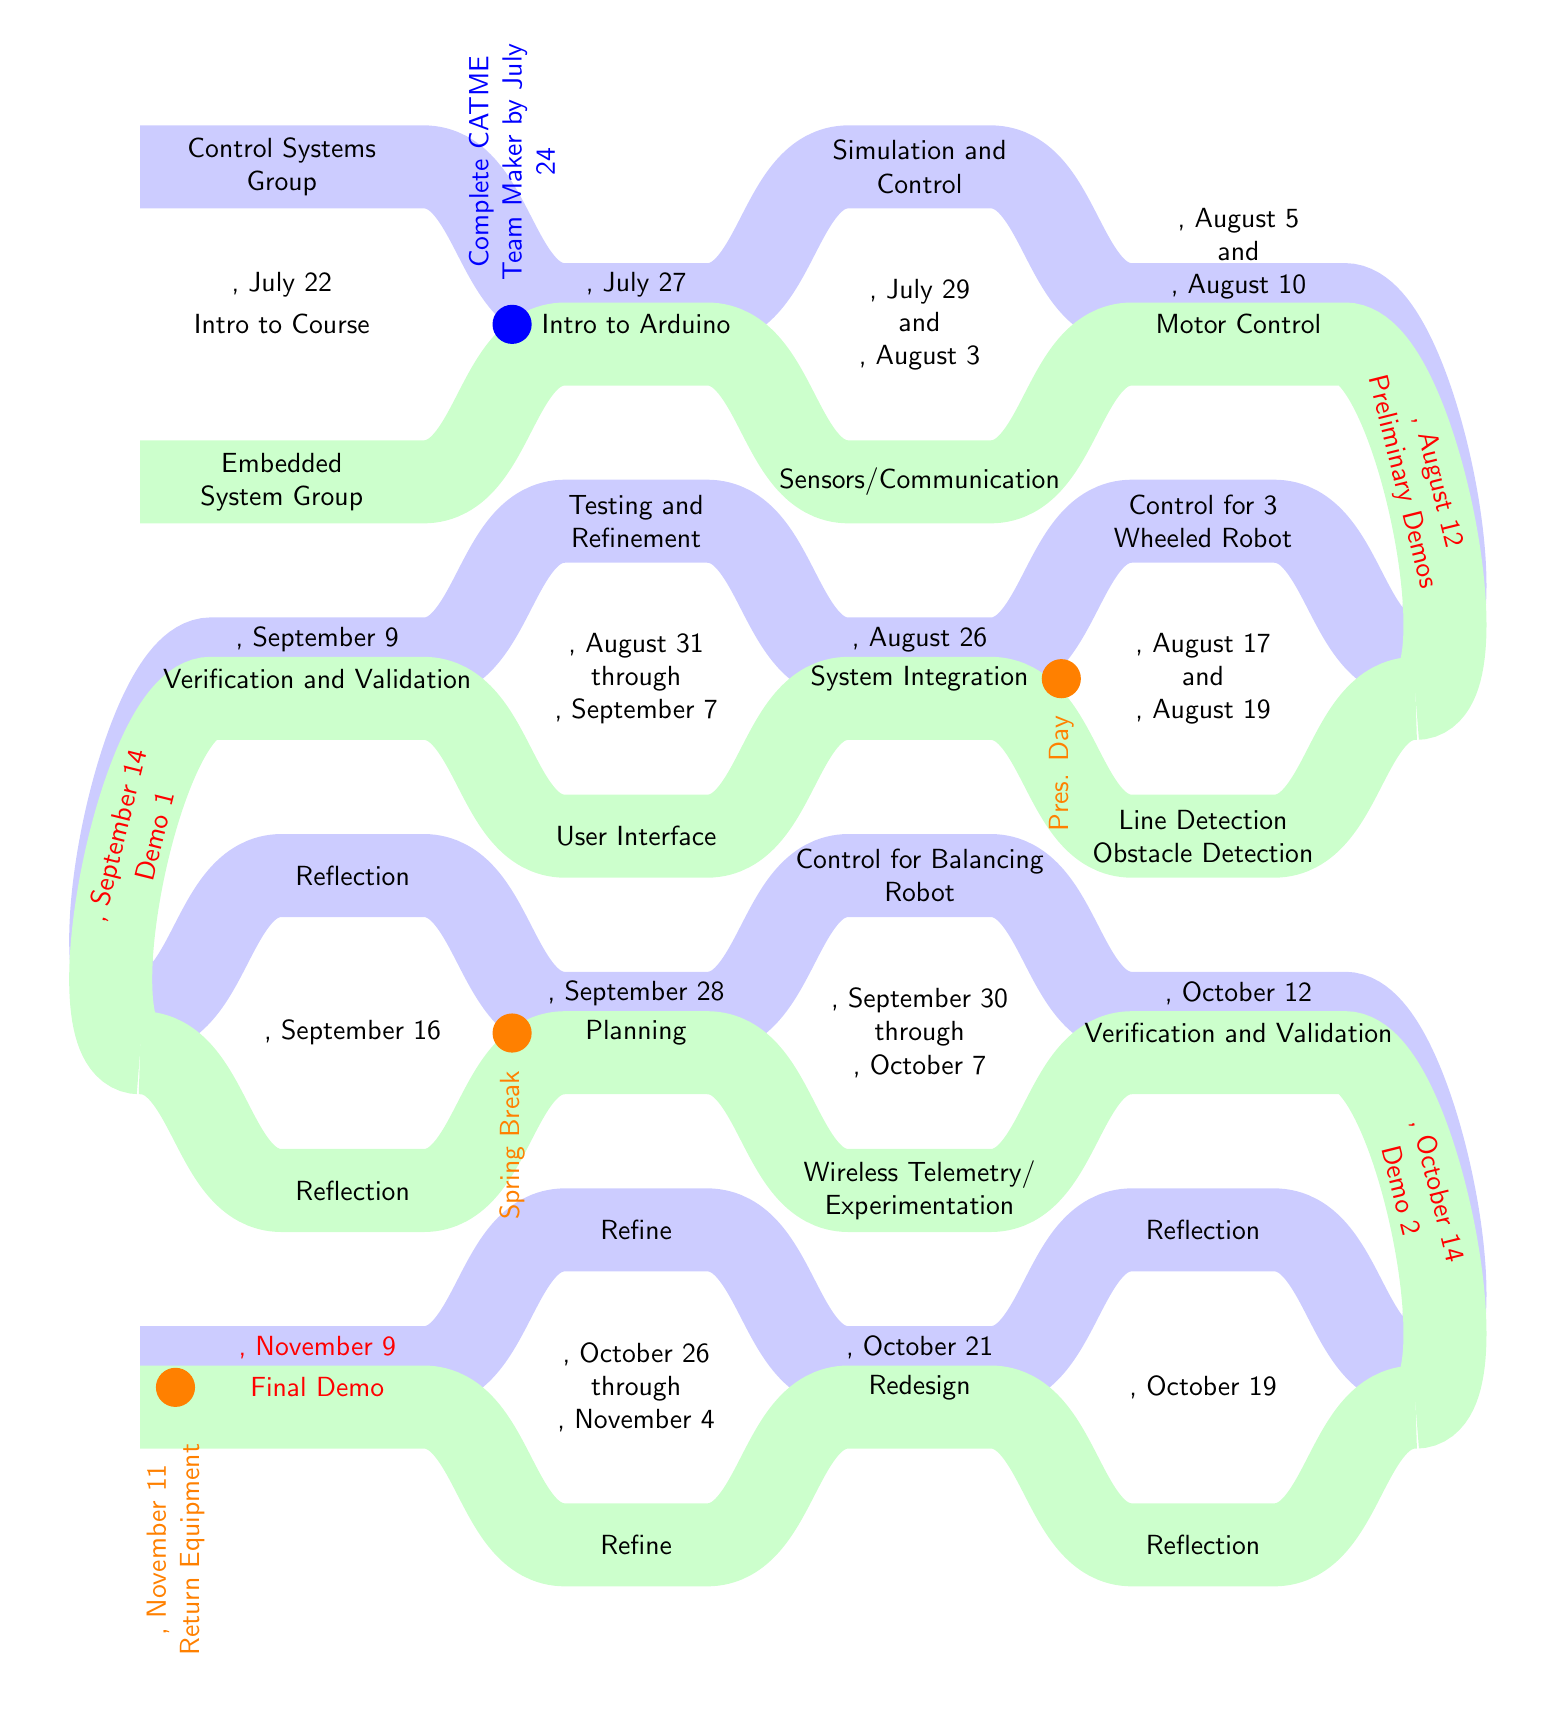
\begin{tikzpicture}[xscale=.9]
% Row 1
\draw[line width=30pt,color=blue!20!white] (-2,0) -- ++(4,0) .. controls ++(1,0) and ++(-1,0) .. ++(2,-1.75) -- ++(2,0) .. controls ++(1,0) and ++(-1,0) .. ++(2,1.75) -- ++(2,0) .. controls ++(1,0) and ++(-1,0) .. ++(2,-1.75) -- ++(3,0) .. controls ++(1,0) and ++(1,0) ..  ++(1,-4.5); 
% Row 2
\draw[line width=30pt,color=blue!20!white] (16,-6.25) .. controls ++(-1,0) and ++(1,0) .. ++(-2,1.75) -- ++(-2,0) .. controls ++(-1,0) and ++(1,0) .. ++(-2,-1.75) -- ++(-2,0) .. controls ++(-1,0) and ++(1,0) .. ++(-2,1.75) -- ++(-2,0) .. controls ++(-1,0) and ++(1,0) .. ++(-2,-1.75) -- ++(-3,0) .. controls ++(-1,0) and ++(-1,0) ..  ++(-1,-4.5); 
% Row 3
\draw[line width=30pt,color=blue!20!white] (-2,-10.75)  .. controls ++(1,0) and ++(-1,0) .. ++(2,1.75) -- ++(2,0) .. controls ++(1,0) and ++(-1,0) .. ++(2,-1.75) - - ++(2,0).. controls ++(1,0) and ++(-1,0) .. ++(2,1.75) -- ++(2,0) .. controls ++(1,0) and ++(-1,0) .. ++(2,-1.75)-- ++(3,0) .. controls ++(1,0) and ++(1,0) ..  ++(1,-4.5); 
% Row 4
\draw[line width=30pt,color=blue!20!white] (16,-15.25) .. controls ++(-1,0) and ++(1,0) .. ++(-2,1.75) -- ++(-2,0) .. controls ++(-1,0) and ++(1,0) .. ++(-2,-1.75) -- ++(-2,0) .. controls ++(-1,0) and ++(1,0) .. ++(-2,1.75) -- ++(-2,0) .. controls ++(-1,0) and ++(1,0) .. ++(-2,-1.75) -- ++(-4,0); 


\draw[line width=30pt,color=green!20!white] (-2,-4) -- ++(4,0) .. controls ++(1,0) and ++(-1,0) .. ++(2,1.75) -- ++(2,0) .. controls ++(1,0) and ++(-1,0) .. ++(2,-1.75) -- ++(2,0) .. controls ++(1,0) and ++(-1,0) .. ++(2,1.75) -- ++(3,0) .. controls ++(1,0) and ++(1,0) ..  ++(1,-4.5); 
\draw[line width=30pt,color=green!20!white] (16,-6.75) .. controls ++(-1,0) and ++(1,0) .. ++(-2,-1.75) -- ++(-2,0) .. controls ++(-1,0) and ++(1,0) .. ++(-2,1.75) -- ++(-2,0) .. controls ++(-1,0) and ++(1,0) .. ++(-2,-1.75) -- ++(-2,0) .. controls ++(-1,0) and ++(1,0) .. ++(-2,1.75) -- ++(-3,0) .. controls ++(-1,0) and ++(-1,0) ..  ++(-1,-4.5);
\draw[line width=30pt,color=green!20!white] (-2,-11.25)  .. controls ++(1,0) and ++(-1,0) .. ++(2,-1.75) -- ++(2,0) .. controls ++(1,0) and ++(-1,0) .. ++(2,1.75) - - ++(2,0).. controls ++(1,0) and ++(-1,0) .. ++(2,-1.75) -- ++(2,0) .. controls ++(1,0) and ++(-1,0) .. ++(2,1.75)-- ++(3,0) .. controls ++(1,0) and ++(1,0) ..  ++(1,-4.5); 
\draw[line width=30pt,color=green!20!white] (16,-15.75) .. controls ++(-1,0) and ++(1,0) .. ++(-2,-1.75) -- ++(-2,0) .. controls ++(-1,0) and ++(1,0) .. ++(-2,1.75) -- ++(-2,0) .. controls ++(-1,0) and ++(1,0) .. ++(-2,-1.75) -- ++(-2,0) .. controls ++(-1,0) and ++(1,0) .. ++(-2,1.75) -- ++(-4,0); 

%
% Row 1
%

\draw (0,0) node {\begin{minipage}{1in}\centering\textsf{Control Systems Group}\end{minipage}};
\draw (0,-1.5) node {\textsf{\sd, \datemonthname\ \thedateday}};
\addtocounter{datenumber}{2}\setdatebynumber{\thedatenumber}
\draw (0,-2) node {\textsf{Intro to Course}};
%
\draw (0,-4) node {\begin{minipage}{1in}\centering\textsf{Embedded System Group}\end{minipage}};
%
% Complete CATME
%
\draw (3.25,-2) node[circle,fill=blue,inner sep=5pt] {} node[rotate=90,right=10pt] {\color{blue}\begin{minipage}{1.25in}\centering\textsf{Complete CATME Team Maker by \datemonthname\ \thedateday}\end{minipage}};
\addtocounter{datenumber}{3}\setdatebynumber{\thedatenumber}
%
\draw (5,-1.5) node {\textsf{\sd, \datemonthname\ \thedateday}};
\addtocounter{datenumber}{2}\setdatebynumber{\thedatenumber}
\draw (5,-2) node {\textsf{Intro to Arduino}};
%
\draw (9,-2) node {\begin{minipage}{1.5in}\centering
\textsf{\sd, \datemonthname\ \thedateday\\
and}\\
\addtocounter{datenumber}{5}\setdatebynumber{\thedatenumber}
\textsf{\sd, \datemonthname\ \thedateday}\end{minipage}};
\draw (9,0) node {\begin{minipage}{1in}\centering\textsf{Simulation and Control}\end{minipage}};
\draw (9,-4) node {\textsf{Sensors/Communication}};

\addtocounter{datenumber}{2}\setdatebynumber{\thedatenumber}
\draw (13.5,-1.1) node {\begin{minipage}{1.5in}\centering
\textsf{\sd, \datemonthname\ \thedateday\\
and}\\
\addtocounter{datenumber}{5}\setdatebynumber{\thedatenumber}
\textsf{\sd, \datemonthname\ \thedateday}\end{minipage}};
\draw (13.5,-2) node  {\textsf{Motor Control}} ;

\addtocounter{datenumber}{2}\setdatebynumber{\thedatenumber}
\draw (16.3,-4) node[rotate=-76] {\color{red}\textsf{\sd, \datemonthname\ \thedateday}};
\draw (15.8,-4) node[rotate=-76] {\color{red}\textsf{Preliminary Demos}};



\addtocounter{datenumber}{5}\setdatebynumber{\thedatenumber}

%
% Row 2
%


\draw (13,-4.5) node {\begin{minipage}{1in}\centering\textsf{Control for 3 Wheeled Robot}\end{minipage}};
\draw (13,-8.5) node {\begin{minipage}{1.5in}\centering\textsf{Line Detection
}\\ \textsf{Obstacle Detection}\end{minipage}};
\draw (13,-6.5) node {\begin{minipage}{1.5in}\centering
\textsf{\sd, \datemonthname\ \thedateday\\
and}\\
\addtocounter{datenumber}{2}\setdatebynumber{\thedatenumber}
\textsf{\sd, \datemonthname\ \thedateday}\end{minipage}};
\addtocounter{datenumber}{5}\setdatebynumber{\thedatenumber}
%
% skip presidents day
%
\draw (11,-6.5) node[circle,fill=orange,inner sep=5pt] {} node[rotate=90,left=10pt] {\textsf{\color{orange}Pres. Day}};

\draw (9,-6.5) node {\textsf{System Integration}};
\addtocounter{datenumber}{2}\setdatebynumber{\thedatenumber}
\draw (9,-6) node {\textsf{\sd, \datemonthname\ \thedateday}};


\draw (5,-4.5) node {\begin{minipage}{1in}\centering\textsf{Testing and Refinement}\end{minipage}};
\draw (5,-8.5) node {\textsf{User Interface}};
\addtocounter{datenumber}{5}\setdatebynumber{\thedatenumber}
\draw (5,-6.5) node {\begin{minipage}{1.5in}\centering
\textsf{\sd, \datemonthname\ \thedateday\\
through}\\
\addtocounter{datenumber}{7}\setdatebynumber{\thedatenumber}
\textsf{\sd, \datemonthname\ \thedateday}\end{minipage}};



\draw (.5,-6.5) node {\textsf{Verification and Validation}};
\addtocounter{datenumber}{2}\setdatebynumber{\thedatenumber}
\draw (0.5,-6) node {\textsf{\sd, \datemonthname\ \thedateday}};


\draw (-1.8,-8.5) node[rotate=76] {\color{red}\textsf{Demo 1}};
\addtocounter{datenumber}{5}\setdatebynumber{\thedatenumber}
\draw (-2.3,-8.5) node[rotate=76] {\color{red}\textsf{\sd, \datemonthname\ \thedateday}};
\addtocounter{datenumber}{2}\setdatebynumber{\thedatenumber}

%
% Row 3
% 

\draw (1,-9) node {\textsf{Reflection}};
\draw (1,-13) node {\textsf{Reflection}};
\draw (5,-11) node {\textsf{Planning}};
\draw (9,-9) node  {\begin{minipage}{1.25in}\centering\textsf{Control for Balancing Robot}\end{minipage}};
\draw (9,-13) node {\begin{minipage}{1.25in}\centering\textsf{Wireless Telemetry/ Experimentation}\end{minipage}};
\draw (13.5,-11) node {\textsf{Verification and Validation}};
\draw (15.8,-13) node[rotate=-76] {\color{red}\textsf{Demo 2}};


\draw (1,-11) node {\begin{minipage}{1.5in}\centering
\textsf{\sd, \datemonthname\ \thedateday}\end{minipage}};
\addtocounter{datenumber}{5}\setdatebynumber{\thedatenumber}

%
% skip spring break
%
\draw (3.25,-11) node[circle,fill=orange,inner sep=5pt] {} node[rotate=90,left=10pt] {\textsf{\color{orange}Spring Break}};
\addtocounter{datenumber}{7}\setdatebynumber{\thedatenumber}


\draw (5,-10.5) node {\textsf{\sd, \datemonthname\ \thedateday}};
\addtocounter{datenumber}{2}\setdatebynumber{\thedatenumber}
\draw (9,-11) node {\begin{minipage}{1.5in}\centering
\textsf{\sd, \datemonthname\ \thedateday\\
through}\\
\addtocounter{datenumber}{7}\setdatebynumber{\thedatenumber}
\textsf{\sd, \datemonthname\ \thedateday}\end{minipage}};
\addtocounter{datenumber}{5}\setdatebynumber{\thedatenumber}
\draw (13.5,-10.5) node {\textsf{\sd, \datemonthname\ \thedateday}};
\addtocounter{datenumber}{2}\setdatebynumber{\thedatenumber}
\draw (16.3,-13) node[rotate=-76] {\color{red}\textsf{\sd, \datemonthname\ \thedateday}};
\addtocounter{datenumber}{5}\setdatebynumber{\thedatenumber}

%
% Row 4
%

\draw (13,-13.5) node {\textsf{Reflection}};
\draw (13,-17.5) node {\textsf{Reflection}};
\draw (9,-15.5) node {\textsf{Redesign}};
\draw (5,-13.5) node {\textsf{Refine}};
\draw (5,-17.5) node {\textsf{Refine}};
\draw (.5,-15.5) node {\textsf{\color{red}Final Demo}};

\draw (13,-15.5) node  {\textsf{\sd, \datemonthname\ \thedateday }};

\addtocounter{datenumber}{2}\setdatebynumber{\thedatenumber}
\draw (9,-15) node {\textsf{\sd, \datemonthname\ \thedateday}};
\addtocounter{datenumber}{5}\setdatebynumber{\thedatenumber}

\draw (5,-15.5) node  {\begin{minipage}{1.5in}\centering
\textsf{\sd, \datemonthname\ \thedateday\\
through}\\
\addtocounter{datenumber}{9}\setdatebynumber{\thedatenumber}
\textsf{\sd, \datemonthname\ \thedateday}\end{minipage}};

\addtocounter{datenumber}{5}\setdatebynumber{\thedatenumber}
\draw (.5,-15) node {\color{red}\textsf{\sd, \datemonthname\ \thedateday}};

\addtocounter{datenumber}{2}\setdatebynumber{\thedatenumber}
\draw (-1.5,-15.5) node[circle,fill=orange,inner sep=5pt] {} node[rotate=90,left=10pt] {\textsf{\color{orange}\begin{minipage}{1.25in}\centering\textsf{\sd, \datemonthname\ \thedateday \\ Return Equipment}\end{minipage}}};


\end{tikzpicture}}
\end{center}



\end{document}

